%%%%%%%%%%%%%%%%%%%%%%%%%%%%%%%%%%%%%%%%%%
% Draft for                              %
% Bayesian Hierarchical Sparse VAR Model %
% for Multiple-Subject Multiple-Session  %
% Resting-state Functional Connectivity  %
%%%%%%%%%%%%%%%%%%%%%%%%%%%%%%%%%%%%%%%%%%



\documentclass[12pt]{elsarticle}
\usepackage{graphicx}
\usepackage{amssymb}
\usepackage{lineno}
\usepackage{geometry}
\geometry{margin=1in}
\usepackage[T1]{fontenc} 
\usepackage{fourier} 
\usepackage[english]{babel} 
\usepackage{amsmath,amsfonts,amsthm} 
\usepackage{sectsty} 
\usepackage{fancyhdr} 
\usepackage{hyperref}
\usepackage{algorithm}
\usepackage{algpseudocode}
\usepackage{afterpage}
\setlength{\headheight}{5pt} 
\setlength\parindent{20pt} 
\newcommand\independent{\protect\mathpalette{\protect\independenT}{\perp}}
\def\independenT#1#2{\mathrel{\rlap{$#1#2$}\mkern2mu{#1#2}}}
\newcommand{\horrule}[1]{\rule{\linewidth}{#1}} 





\begin{document}
	
	\begin{frontmatter}
		
		\title{A Bayesian hierarchical sparse VAR model for multiple-subject multiple-session resting-state effective connectivity}
		
		\author{Feihan Lu}
		
		
		\begin{abstract}
			Vector autoregressive (VAR) models provide a convenient yet informative framework for learning associations among nodes in graphs. 
			They have been widely applied to a variety of studies, including effective connectivity among brain networks or regions of interest (ROI).  
			However, existing applications have several limitations. 
			First, models that consider connectivity structures for single or multiple subjects within only one imaging session has been developed, and none has been proposed to handle multiple-subject multiple-session data.
			Second, in many sparse VAR models, the covariance matrix of the innovation process has been explicitly or implicitly assumed to be diagonal, which, despite of its convenience, is not accurate enough for many real practices.   
			In this project, a new Bayesian hierarchical sparse VAR model is proposed for resting-state effective connectivity that generalizes the these limitations:
			(1). It can be applied to multiple-subject multiple-session data and is capable of simultaneous inference about population-level, subject-level and session-level connectivity over moderately large number of ROIs; 
			(2). By adopting the doubly adaptive Elastic-net Lasso prior \cite{Gefang}, this model is able to obtain sparse estimates without assuming any special structure of the error covariance matrix. 
			The model is applied to the Human Connectome Project (HCP) data, and  distinct connectivity among 15 ROIs over 7 brain networks is revealed.
		\end{abstract}
		
		
	\end{frontmatter}
	
	
	%\linenumbers
	
	
	
	\section{Introduction}
	Vector Autoregressive (VAR) models have been widely applied to a variety of fields of study, including macroeconomics, finance, etc. 
	One attractive nature of these models is the ease to investigate lagged causations among distinct factors, which are represented by multivariate time series.
	Recently, they have also become a rising star for neuron-scientists to characterize human brain connectivity structures among different regions of interest (ROI) across the brain \cite{Gorrostieta} \cite{Harrison}. 
	In particular, one important application is to the functional magnetic resonance imaging (fMRI) time series data, where the fMRI scanner keeps tract of the blood oxygenation across different regions of the brain, called blood oxygenation level dependence (BOLD) responses, which represent the underlying neurophysiology activities within those regions.
	The VAR models provide an intuitive and promising tool that captures the causations, or \textit{effective connectivity}, among those brain regions over different time frames. 
	
	
	While classical frequentists' approaches such as maximum likelihood estimate (MLE) allow convenient estimation of the VAR models, they are at high risk to result in high variance of the estimates and may even produce spurious estimates when the number of regions in the model is large. 
	A natural remedy to solve such issue is to introduce the Bayesian frameworks that induce shrinkage and/or sparsity into the estimation of the model coefficients, which may slightly produce bias but greatly reduce variance, leading to decreased total estimation inaccuracy.
	In the fMRI literature, examples include \cite{Harrison}, who proposed a Bayesian VAR model with Normal prior on the parameters, a general form of the ridge regression type of shrinkage, and \cite{Gorrostieta}, who proposed a hierarchical model with Elastic-net type of regularization, in the spirit of \cite{Lin}, to study effective connectivity across multiple subjects. 
	In other fields of study, different Bayesian sparse VAR applications are also plausible, including \cite{Gefang}'s doubly adaptive Elastic-net VAR shrinkage, which is used to study the causal relationships among macroeconomic factors.
	
	
	While those Bayesian models worked well on certain situations, there are several limitations. 
	First, some of them assume special structures, such as diagonal structure, for the variance-covariance matrix of the innovation process. 
	While this assumption might be computationally handy, it might not be valid for more general situations and may suffer from estimation inaccuracy.
	Second, these methods are suitable for the data of single or multiple subjects at one single fMRI scanning session. 
	However, when there are repeated fMRI scans of the same subject(s) across multiple sessions, those models become restricted and insufficient.
	Third, the applications of those models remain low-dimensional, in that there are only a small number of ROI's (such as 5 or 6) being considered among a small number of subjects (such as 20).
	While this might lessen the computational burden and provide reliable insights for small-scaled connectivity, it would be more practical and meaningful to extend to larger-scaled inference with greater number of ROI's on larger sample sizes.
	
	
	In this project, I propose a hierarchical model that overcomes those limitations. 
	This model extends the existing methods to cope with multiple-subject multiple-session data, and aims at simultaneous inference about population-level, subject-level and session-level effective connectivity over moderately large number of ROI's and subjects. 
	By adopting the doubly adaptive Elastic-net prior proposed by \cite{Gefang}, the model is able to induce sparsity into the estimation of population-level coefficients under no assumption of any special structure of the error covariance matrix.
	The model is applied to resting-state fMRI time series, for which the subjects under the scans are at rest and take no tasks.
	
	
	
	\section{Method}
	
	Suppose we have $N$ subjects, each of whom has $S$ sessions of fMRI scans. 
	Each scan is run for $T$ time points and BOLD responses for each of the time points are recorded, usually over a large number of voxels across the entire brain.
	Those voxels are grouped into $B$ pre-defined ROI's, and mean BOLD time series within those ROI's are calculated.
	The gold is to investigate the causal relationships among those mean BOLD time series. 
	To do this, let $\boldsymbol{y}_{njt}=(y_{njt1},...,y_{njtB})^T$ be a column vector of length $B$ representing the mean BOLD responses across $B$ ROI's at time $t=1, ..., T$ for subject $n=1,...,N$ for session $s=1,...,S$.  
	Then the Bayesian VAR($p$) model assumes 
	\begin{equation} \label{eq:1}
		\boldsymbol{y}_{njt} = \sum_{i=1}^p A_{nji} \boldsymbol{y}_{nj,t-i}+ \boldsymbol{e}_{njt},  t=p+1,...,T
	\end{equation}
	where $A_{nji}, i=1,...,p$ is a $B\times B$ coefficient matrix representing the lag-$i$ effect, and $ \boldsymbol{e}_{njt}$ is the innovation process assumed to follow i.i.d. multivariate Normal distribution with mean $\boldsymbol{0}$ and precision matrix $\Lambda: \boldsymbol{e}_{njt} \sim MN(\boldsymbol{0}, \Lambda^{-1})$.
	The model can be concisely written in the matrix form of
	\begin{equation} \label{eq:2}
		\boldsymbol{y}_{nj} = \left(H_{nj}^T \otimes I_B \right)\boldsymbol{w}_{nj} + \boldsymbol{e}_{nj}
	\end{equation}
	where
	\[\boldsymbol{y}_{nj}=
	\begin{pmatrix}
	\boldsymbol{y}_{nj,p+1}\\
	\vdots \\
	\boldsymbol{y}_{njT}
	\end{pmatrix}
	\]
	is the response variable, 
	\[H_{nj}=
	\begin{pmatrix}
	\boldsymbol{y}_{njp} & \cdots  & \boldsymbol{y}_{nj,T-1}\\
	\vdots &  \ddots & \vdots\\
	\boldsymbol{y}_{nj1} & \cdots & \boldsymbol{y}_{nj,T-p}
	\end{pmatrix}
	\]
	is the regressors,
	\[\boldsymbol{w}_{nj}=vec([A_{nj1},...,A_{njp}])\]
	is the vectorized coefficients of length $B^2p$, 
	\[\boldsymbol{e}_{nj} \sim MN(\textbf{0}, I_{T-p} \otimes \Lambda^{-1})\]
	is the stacked error term, $I_k$ is a $k\times k$ identity matrix, and $\otimes$ stands for Kronecker product.
	Here we assume that the precision matrix $\Lambda$ is the same for all subjects and all sessions, but the coefficient vector $\boldsymbol{w}_{nj}$ is unique for each subject and each session.
	Specifically, we assume that the coefficient vector for the $n$-th subject and the $j$-th session is composed of 3 parts:
	\begin{equation} \label{eq:3}
		\boldsymbol{w}_{nj}=\boldsymbol{w}+\boldsymbol{v}_{n} + \boldsymbol{u}_{j}
	\end{equation}
	where $\boldsymbol{w}$ is the population-level effect that is the same for all subjects and all sessions, $\boldsymbol{v}_{n}$ is the subject-level effect specifically for subject $n$, and $\boldsymbol{u}_{j}$ is the session-level effect specifically for session $j$. 
	
	For the population-level effect, we adopt the doubly adaptive Elastic-net prior proposed by \cite{Gefang}.
	Specifically, we assume that $\boldsymbol{w}$ follows multivariate Normal distribution with mean $\boldsymbol{0}$ and diagonal precision matrix $D$: 
	\begin{equation} \label{eq:4}
		\boldsymbol{w} | D  \sim MN \left( \boldsymbol{0},  D^{-1} \right)
	\end{equation}
	where $D$ depends on hyper-parameters $2\tau_k^2$ and $\lambda_{2,k}, k=1,...,B^2p$:
	\begin{equation} \label{eq:5}
		D=diag\left( \lambda_{2,1}+\frac{1}{2\tau_1^2},...,\lambda_{2,B^2p}+\frac{1}{2\tau_{B^2p}^2}\right)
	\end{equation}
	and each $2{\tau}_k^2$ follows Exponential distribution with rate parameter $\frac{2\xi_k^2}{\lambda_{1,k}^2}$:
	\begin{equation} \label{eq:6}
		2\tau_k^2 | 2\xi_k^2, \lambda_{1,k}^2 \sim Exp\left( \frac{2\xi_k^2}{\lambda_{1,k}^2}\right)
	\end{equation}
	where $\xi_k^2, k=1,...,B^2p$, depends on the error precision matrix $\Lambda$ through:
	\begin{equation} \label{eq:7}
		\xi_k^2=M_{k,k}-\left(M_{k,k+1},...,M_{k,B^2p}\right)
		{\begin{pmatrix}
				M_{k+1,k+1} & \cdots & M_{k+1, B^2p} \\
				\vdots & \ddots & \vdots \\
				M_{B^2p,k+1}  & \cdots & M_{B^2p,B^2p} 
			\end{pmatrix}}^{-1}
			\begin{pmatrix}
				M_{k,k+1}\\
				\vdots \\
				M_{k,B^2p}
			\end{pmatrix}
		\end{equation}
		\begin{equation} \label{eq:8}
			M=I_{Bp} \otimes \Lambda^{-1}
		\end{equation}
		and $\lambda_{1,k}^2$ and $\lambda_{2,k}, k=1,...,B^2p$ follow two i.i.d. Gamma distributions:
		\begin{equation} \label{eq:9}
			\lambda_{1,k}^2 \sim Gamma(\mu_1, \nu_1)
		\end{equation}
		\begin{equation} \label{eq:10}
			\lambda_{2,k} \sim Gamma(\mu_2, \nu_2)
		\end{equation}
		where $\mu_1, \nu_1, \mu_2, \nu_2$ are corresponding mean and degree of freedom parameters, which are assumed to be known.
		Here, $\lambda_{1,k}^2$ and $\lambda_{2,k}$ represent the L1 and L2 tuning parameters for the $k$-th element of $\boldsymbol{w}$.
		It can be shown that the conditional distribution of each of the element of $\boldsymbol{w}$ given the error precision matrix $\Lambda$ is composed of a Normal distribution and a Laplace distribution.
		In other words, this prior generalizes the adaptive LASSO and provides adaptive shrinkage for the Elastic-net regularization. 
		Note that conditioning on the error precision matrix $\Lambda$ is important as it ensures unimodal posterior distribution for each of the elements of $\boldsymbol{w}$\cite{Park}.
		
		
		For the subject-level and session-level effects, we apply conjugate i.i.d. multivariate Normal priors with mean $\boldsymbol{0}$ and diagonal precision matrices $\Theta_v$ and $\Theta_u$:
		\begin{equation} \label{eq:11}
			\boldsymbol{v}_{n}|\Theta_v \sim MN \left( \boldsymbol{0}, \Theta_v^{-1} \right)
		\end{equation}
		\begin{equation} \label{eq:12}
			\boldsymbol{u}_{j}|\Theta_u \sim MN \left( \boldsymbol{0}, \Theta_u^{-1} \right)
		\end{equation}
		for $n=1,...,N$ and $j=1,...,J$, where
		\begin{equation} \label{eq:13}
			\Theta_v = diag(\theta_{v1},...,\theta_{v,B^2p})
		\end{equation}
		\begin{equation} \label{eq:14}
			\Theta_u = diag(\theta_{u1},...,\theta_{u,B^2p})
		\end{equation}
		with Gamma hyperpriors on each of the diagonal elements $\theta_{vk}$ and $\theta_{uk}, k=1,...,B^2p$:
		\begin{equation} \label{eq:15}
			\theta_{vk} \sim Gamma(k_1, s_1)
		\end{equation}
		\begin{equation} \label{eq:16}
			\theta_{uk} \sim Gamma(k_2, s_2)
		\end{equation}
		where $k_1, s_1, k_2, s_2$ are known mean and degree of freedom parameters.
		
		Finally, we utilize conjugate Wishart distribution for the error precision matrix $\Lambda$:
		\begin{equation} \label{eq:17}
			\Lambda \sim Wishart(K, \nu)
		\end{equation}
		where $K$ is the $B \times B$ scale matrix and $\nu$ is degree of freedom parameter, both assumed to be known. 
		We use Axillary Gibbs Sampler along with 2-Stage Method-of-Moments-type initial values to draw from posterior distribution (see Appendix for details). 
		
		
		
		
		
		
		
		
		\section{Real example}
		The example to apply our model to is the Human Connectome Project  \url{http://www.humanconnectomeproject.org}, which is an extensive research database for human brain connectivity studies. 
		We picked a dataset containing 50 subjects with 4 rest-state fMRI sessions on 15 pre-defined ROI's across 1200 time points (separated by 2 seconds) within each session. 
		Those ROI's are selected across 7 brain networks including subcortical, auditory, somatomotor cortex, visual, cognitive-control, default mode and cerebellum. 
		One remarkable feature about this dataset is its high dimensionality. 
		For a VAR model of order $p$, there are more than 12,000$p$ parameters.
		Fortunately, by adopting auxiliary variables and utilizing Method-of-Moments-like estimates as initial values in the Gibbs Sampler algorithm, we are able to efficiently draw from posterior distribution even with limited computational resources in both time and memory.
		
		
		A VAR($1$) model is fitted to the example data.
		Figure \ref{pop} shows the posterior modes of the population-level effects, stacking the vector $\boldsymbol{w}$ back into $B \times B$ matrix.
		Using posterior modes as point estimates is an approach to induce sparsity, which is shown to be equivalent to the estimates given by the penalized likelihood methods such as LASSO \cite{Park}. 
		Here, R1 to R7 represents the 7 brain networks, and the $ij$-th cell of the matrix in the plot represents the lag-1 effect of the $i$-th ROI on the $j$-th ROI.
		Note that we are particularly interested in the cross-relationship among distinct ROI's and networks, and so only off-diagonal elements in the matrix are shown in the graph.
		One can see that many of the cells are white, representing sparse estimates zeroed out by the Elastic-net prior.
		Some of the cells are darker blue, showing strong negative effects of the somatomotor cortex (R3) and defauld-mode network (R6) on the subcortical network (R1).
		Moreover, there seem to be strong positive effects among the ROI's within the subcortical network and defauld-mode network.
		
		Figure \ref{session} shows the posterior modes of the session-level effects by stacking the estimated vector $\boldsymbol{u}_j, j=1,...,4$ back into matrices. 
		One can see that the majority of the cells are white, meaning no effects among the ROI's, and this pattern is consistent over all 4 sessions.
		This suggests weak variability in brain connectivity due to the difference in sessions.
		
		On the other hand, there seem to be much greater subject-level effects and larger variabilities among different subjects, compared to the session-level counterparts. 
		Figure \ref{subject} shows the posterior modes of the subject-level effects for the first 4 subjects in the dataset for illustration.
		One can see that there are much greater positive or negative effects among the ROI's, and the relationships vary drastically across distinct subjects, although some of the cells (e.g., those in the bottom-left corner) seem to be consistently zero. 
		
		
		Combining the two findings, it seems to suggest that people's brains are connected in widely different ways, but the connectivity for each individual subject remains consistent over time. 
		Figure \ref{variability} shows the estimated standard deviation of the session-level and subject-level coefficients (i.e., stacking back the squared-root of the inverse of the diagonal elements of $\Theta_u$ and $\Theta_v$ into matrices), along with the proportion of the session-level variance in the sum of session- and subject-level variances.
		One can see that most elements of the session-level variance is tiny, compared to those of the subject-level variance, confirming the finding that the majority of the variability in human brain connectivity is due to the difference across individual subjects, not to the difference in sessions.
		
		
		
		
		\section{Summary}
		In summary, we propose a Bayesian hierarchical model that is a new generalization for characterizing multiple-subject multiple-session effective connectivity.
		The proposed model is capable of simultaneous inference about population-level, session-level and subject-level connectivity.
		It is a breakthrough in the fMRI literature in that it allows the researchers to understand substantively what drives the difference in human brain connectivity across subjects \textit{and} across sessions.
		The model found strong negative and positive effects among several distinct regions of interest across 7 brain networks in the population level.
		It also provided insights of the within-subject and between-subject variabilities and found that the total variability is largely explained by difference between subjects.
		It relies on no special assumption about the error covariance matrix, and is thus flexible for general situations.
		Last but not least, implemented by Auxiliary Gibbs Sampler with 2-Stage Method-of-Moments-like initial values, this model is able to handle large dataset and high-dimensionality.
		In the future, it would be of interest to extend the model to even larger-scaled datasets, with larger sample sizes, greater number of ROI's, and/or deeper levels of inference, such as a whole-brain voxel-level inference on the complete sample of Human Connectome Project database. 
		In that case, one would need more sophisticated computational strategies including parallel computing techniques such as the consensus Monte Carlo algorithm \cite{Scott}.
		
		
		\section{Appendix}
		
		\subsection{Auxiliary variables}
		Gibbs Sampler algorithm is implemented to draw from the posterior distribution of the proposed model. 
		Note that there are high correlations among the parameters, which is a common phenomenon in many hierarchical models.
		To cope with this issue, auxiliary variables are introduced. 
		Specifically, instead of assuming $\boldsymbol{w}_{nj} = \boldsymbol{w} + \boldsymbol{v}_n + \boldsymbol{u}_j$ in Eq.\ref{eq:3}, we assume
		\begin{equation} \label{eq:18}
			\boldsymbol{w}_{nj} = \boldsymbol{w} + \boldsymbol{\alpha}*\boldsymbol{v}_{n} + \boldsymbol{\beta}*\boldsymbol{u}_{j}
		\end{equation}
		where $\boldsymbol{\alpha}$ and $\boldsymbol{\beta}$ are auxiliary vector-valued variables of length $B^2p$, assumed to follow multivariate Normal distributions
		\begin{equation} \label{eq:19}
			\boldsymbol{\alpha} \sim  MN(\boldsymbol{0},aI)
		\end{equation}
		\begin{equation} \label{eq:20}
			\boldsymbol{\beta} \sim  MN(\boldsymbol{0},bI)
		\end{equation}
		where $a$ and $b$ are constants, and $*$ stands for element-wise multiplication. 
		In this specification, the true subject- and session-level effects become 
		\begin{equation} \label{eq:21}
			\boldsymbol{v}_{n}^{*} = \boldsymbol{\alpha} * \boldsymbol{v}_{n}
		\end{equation}
		\begin{equation} \label{eq:22}
			\boldsymbol{u}_{j}^{*} = \boldsymbol{\beta} * \boldsymbol{u}_{j}
		\end{equation}
		and the true precision of those effects (compared with Eq \ref{eq:13} and \ref{eq:14}) become
		\begin{equation} \label{eq:23}
			\theta_{vk}^{*} = \alpha_k^{-2}\theta_{vk} 
		\end{equation}
		\begin{equation} \label{eq:24}
			\theta_{uk}^{*} = \beta_k^{-2}\theta_{uk} 
		\end{equation}
		for $k=1,...,B^2p$, where  $\alpha_k$ and $\beta_k$ are the $k$-th elements of $\boldsymbol{\alpha}$ and $\boldsymbol{\beta}$.
		Note that we are only interested in the posterior inference of $\boldsymbol{v}_{n}^{*}$,  $\boldsymbol{u}_{j}^{*}$, $\theta_{vk}^{*}$, and $\theta_{uk}^{*}$.  
		
		
		
		\subsection{2-Stage Method-of-Moments-like initial values}
		Besides adopting auxiliary variables to break the correlations among the parameters and fasten posterior sampling speed, one can also adjust initial values to boost the MCMC procedure.
		In our practice, we develop a 2-Stage Method-of-Moments-like estimates as starting points for population-, session- and subject-level effects. 
		The first stage is to obtain the MLE's of the coefficients $\hat{\boldsymbol{w}}_{nj}$ for $n=1,...,N$ and $j=1,...,J$: 
		
		\begin{equation} \label{eq:25}
			\hat{\boldsymbol{w}}_{nj} = \left[ \left( H_{nj}H_{nj}^{T}\right)^{-1}H_{nj}\otimes I_{B} \right] \boldsymbol{y}_{nj}
		\end{equation}
		
		The second stage is to use these MLE's to form initial values for the population-, session-, and subject-level coefficients. 
		Specifically,
		\[\hat{\boldsymbol{w}} = \frac{1}{NJ} \sum_{n=1}^{N} \sum_{j=1}^{J} \hat{\boldsymbol{w}}_{nj}\]
		\[ \hat{\boldsymbol{v}}_{n} = \frac{1}{J} \sum_{j=1}^{J}(\hat{\boldsymbol{w}}_{nj}-\hat{\boldsymbol{w}})\]
		\[\hat{\boldsymbol{u}}_{j}=\frac{1}{N}\sum_{n=1}^{N}(\hat{\boldsymbol{w}}_{nj}-\hat{\boldsymbol{w}})\]
		Using these initial values, the Gibbs Sampler algorithm is greatly boosted and computational time reduced by 60\%. 
		
		
		
		
		
		
		\subsection{Full conditional distributions}
		To draw from posterior distribution using Gibbs Sampler, one draws each parameter from its conditional distribution given all other parameters at their current values one at the time. 
		Let $g(\cdot)$ denote conditional distribution of one parameter given others. 
		We now give the full conditional distributions of all parameters.
		
		\begin{enumerate}
			
			\item  $g\left(\boldsymbol{w}\right)=MN\left(M_{w},\, S_{w}^{2}\right)$, where
			\[S_{w}^{2}=\left[ \sum_{n=1}^{N} \sum_{j=1}^{J} \left(H_{nj}H_{nj}^{T}\right) \otimes \Lambda + D \right]^{-1}\]
			\[M_{w} = S_{w}^{2} \left[ \sum_{n=1}^{N} \sum_{j=1}^{J} \left( H_{nj}H_{nj}^{T} \right) \otimes \Lambda \left( \hat{\boldsymbol{w}}_{nj} - \boldsymbol{\alpha} * \boldsymbol{v}_{n} - \boldsymbol{\beta} * \boldsymbol{u}_{j} \right) \right] \]
			where $\hat{\boldsymbol{w}}_{nj}$ is the MLE given by Eq.\ref{eq:25}.
			
			\item $g\left(\boldsymbol{v}_{n}\right)=MN\left(M_{v_{n}},\, S_{v_{n}}^{2}\right), n=1,...,N$, where
			\[S_{v_{n}}^{2}=\left[diag(\boldsymbol{\alpha})\sum_{j=1}^{J} \left(H_{nj}H_{nj}^{T}\right) \otimes \Lambda diag(\boldsymbol{\alpha})+\Theta_{v})\right]^{-1}\]
			\[
			M_{v_{n}} = S_{v_{n}}^{2} \left[diag(\boldsymbol{\alpha}) \sum_{j=1}^{J} \left(H_{nj}H_{nj}^{T}\right) \otimes \Lambda \left(\hat{\boldsymbol{w}}_{nj} - \boldsymbol{w} - \boldsymbol{\beta}*\boldsymbol{u}_{j}\right)\right]
			\]
			
			\item $g\left(\boldsymbol{u}_{j}\right)=MN\left(M_{u_{j}},\, S_{u_{j}}^{2}\right), j=1,...,J$, where
			\[
			S_{u_{j}}^{2} = \left[diag(\boldsymbol{\beta}) \sum_{n=1}^{N} \left(H_{nj}H_{nj}^{T}\right) \otimes \Lambda  diag(\boldsymbol{\beta}) + \Theta_{u} \right]^{-1}
			\]
			\[
			M_{u_{j}} = S_{u_{j}}^{2} \left[ diag(\boldsymbol{\beta}) \sum_{n=1}^{N}\left(H_{nj}H_{nj}^{T} \right) \otimes \Lambda \left(\hat{\boldsymbol{w}}_{nj} - \boldsymbol{w} - \boldsymbol{\alpha} * \boldsymbol{v}_{n} \right)\right]
			\]
			
			
			\item $g\left(\boldsymbol{\alpha}\right)=MN\left(M_{\alpha},\, S_{\alpha}^{2}\right)$, where
			\[
			S_{\alpha}^{2} = \left[ \sum_{n=1}^{N} diag(\boldsymbol{v}_{n}) \sum_{j=1}^{J} \left(H_{nj}H_{nj}^{T}\right) \otimes \Lambda  diag(\boldsymbol{v}_{n}) + aI\right]^{-1}
			\]
			\[
			M_{\alpha} = S_{\alpha}^{2} \left[\sum_{n=1}^{N} diag(\boldsymbol{v}_{n}) \sum_{j=1}^{J} \left(H_{nj}H_{nj}^{T}\right) \otimes \Lambda \left(\hat{\boldsymbol{w}}_{nj} - \boldsymbol{w} - \boldsymbol{\beta} * \boldsymbol{u}_{j} \right)\right]
			\]
			
			
			\item $g\left(\boldsymbol{\beta}\right)=MN\left(M_{\beta},\, S_{\beta}^{2}\right)$, where
			\[ 
			S_{\beta}^{2} = \left[\sum_{j=1}^{J} diag(\boldsymbol{u}_{j}) \sum_{n=1}^{N} \left(H_{nj}H_{nj}^{T}\right) \otimes \Lambda  diag(\boldsymbol{u}_{j})+bI\right]^{-1}
			\]
			\[
			M_{\beta} = S_{\beta}^{2} \left[ \sum_{j=1}^{J} diag(\boldsymbol{u}_{j}) \sum_{n=1}^{N} \left(H_{nj}H_{nj}^{T}\right) \otimes \Lambda \left(\hat{\boldsymbol{w}}_{nj} - \boldsymbol{w} - \boldsymbol{\alpha} * \boldsymbol{v}_{n} \right)\right]
			\]
			
			
			\item $g\left(\theta_{vk}\right)=Gamma(k_{v}, s_{vk}), k=1,...,B^2p$, where
			\[k_{v}=\frac{N}{2}+k_{1}\]
			\[s_{vk} = \left(\frac{1}{2}\sum_{n=1}^{N} {v}_{nk}^{2} + \frac{1}{s_{1}}\right)^{-1}
			\]
			where ${v}_{nk}$ is the $k$-th element of $\boldsymbol{v}_{n}$.
			
			\item $g\left(\theta_{uk}\right)=Gamma(k_{u},s_{uk}), k=1,...,B^2p$, where 
			\[k_{u}=\frac{J}{2}+k_{2}\]
			\[s_{uk}=\left(\frac{1}{2}\sum_{j=1}^{J}{u}_{jk}^{2} + \frac{1}{s_{2}} \right)^{-1}
			\]
			where ${u}_{jk}$ is the $k$-th element of $\boldsymbol{u}_{j}$.
			
			
			\item $g(\lambda_{1,k}^{2}) = Gamma\left(\mu_{\lambda_{1,k}^{2}},\nu_{\lambda_{1,k}^{2}}\right), k=1,...,B^2p$, where
			\[\nu_{\lambda_{1,k}^{2}}=\nu_{1}+2\]
			\[\mu_{\lambda_{1,k}^{2}} = \frac{(\nu_{1}+2)(\mu_{1}\xi_{k}^{2})}{\nu_{1}\xi_{k}^{2}+2\tau_{k}^{2}\mu_{1}}\]
			
			
			
			\item $g(\lambda_{2,k}) = Gamma\left(\mu_{\lambda_{2,k}},\nu_{\lambda_{2,k}}\right), k=1,...,B^{2}p$, where
			\[\nu_{\lambda_{2,k}}=\nu_{2}+1\]
			\[\mu_{\lambda_{2,k}}=\frac{(\nu_{2}+1)\mu_{2}}{\nu_{2}+w_{k}^{2}\mu_{2}}\]
			where $w_{k}$ is the $k$-th element of $\boldsymbol{w}$.
			
			
			
			\item $g\left(\Lambda\right) = Wishart(S_{\Lambda},\nu_{\Lambda})
			$, where
			\[\nu_{\Lambda}=(T-p)NJ+\nu+2Bp\]
			\[S_{\Lambda} = \left[ \sum_{n=1}^{N} \sum_{j=1}^{J} S_{nj} + K^{-1} + 2QQ^{T} \right] ^{-1}\]
			where
			\[S_{nj} =(Y_{nj}-W_{nj}H_{nj})(Y_{nj}-W_{nj}H_{nj})^{T}\]
			is the residual matrix of the $n$-th subject and $j$-th session,
			\[
			Y_{nj} =
			\begin{pmatrix}
			\boldsymbol{y_{nj,p+1}} & \cdots & \boldsymbol{y_{nj,T}}
			\end{pmatrix}
			\]
			is a $B \times (T-p)$ matrix,
			\[W_{nj} = vec^{-1} \left( \boldsymbol{w} + \boldsymbol{\alpha}*\boldsymbol{v}_{n} + \boldsymbol{\beta}*\boldsymbol{u}_{j} \right)\]
			where $vec^{-1}(\cdot)$ means stacking the $B^2p$- coefficient vector back into a $B \times Bp$ matrix, and 
			\[
			Q = 
			\begin{pmatrix}
			\gamma_1 & \cdots & \gamma_{(Bp-1)B+1} \\
			\vdots & \ddots & \vdots \\
			\gamma_{B} & \cdots & \gamma_{B^2p}
			\end{pmatrix}
			\]
			is a $B \times Bp$ matrix composed of $\gamma_k, k=1,...,B^2p$, which depend on $2\tau_k^2, k=1,...,B^2p$ and $\Lambda$ through
			\[\tau_{B^2p} \lambda_{1,B^2p} = \gamma_{B^2p}\]
			\[\tau_{k} \lambda_{1,k} = \gamma_{k}+\boldsymbol{m}_{k}\left(\gamma_{k+1},...,\gamma_{B^{2}p}\right)^{T}\]
			for $k=1,...,B^2p-1$, where
			\[
			\boldsymbol{m}_{k} = \left(M_{k,k+1},...,M_{k,B^2p}\right)
			{\begin{pmatrix}
				M_{k+1,k+1} & \cdots & M_{k+1, B^2p} \\
				\vdots & \ddots & \vdots \\
				M_{B^2p,k+1}  & \cdots & M_{B^2p,B^2p} 
				\end{pmatrix}}^{-1}
			\]
			
			
			
			\item $g(\frac{1}{2\tau_{k}^{2}}) =\sqrt{\frac{b_{k}}{2\pi}} \left( \frac{1}{2\tau_{k}^{2}} \right)^{-\frac{3}{2}}exp\left\{ -\frac{b_{k}\left(\frac{1}{2\tau_{k}^{2}}-a_{k}\right)^{2}} {2a_{k}^{2}\frac{1}{2\tau_{k}^{2}}}\right\}, k=1,...,B^2p$, where
			\[a_{k}=\sqrt{\frac{\lambda_{1,k}^{2}}{w_{k}^{2}\xi_{k}^{2}}}\]
			\[b_{k}=\frac{\lambda_{1,k}^{2}}{\xi_{k}^{2}}\]
			Note that it is hard to analytically write out the conditional distribution of $2\tau_{k}^{2}$, but \cite{Park} has shown that $g(\frac{1}{2\tau_{k}^{2}})$ is Inverse-Gaussian distribution. 
			Therefore, we draw $\frac{1}{2\tau_{k}^{2}}$ first from $g(\frac{1}{2\tau_{k}^{2}})$ and then transform back to get $2\tau_{k}^{2}$.
			
			
		\end{enumerate}
		
		
		
		
		
		
		
		
		
		
		% Figures here
		\afterpage{
			\begin{figure}[h]
				\caption{Posterior modes of population-level effects for 15 ROI's across 7 brain networks}
				\centering
				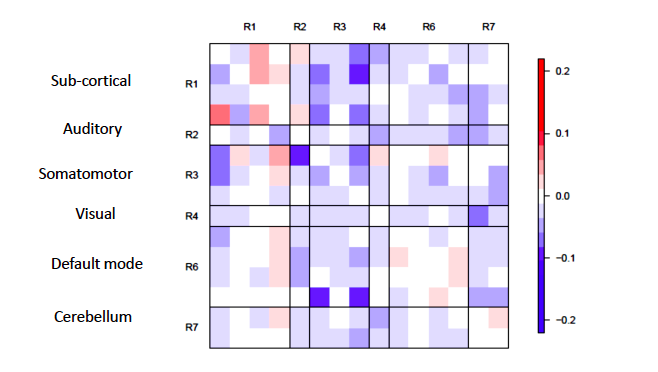
\includegraphics[width=5in]{pop.png}
				\label{pop}
			\end{figure} 
			\clearpage}
		
		\afterpage{
			\begin{figure}[h]
				\caption{Posterior modes of session-level effects for 15 ROI's across 7 brain networks}
				\centering
				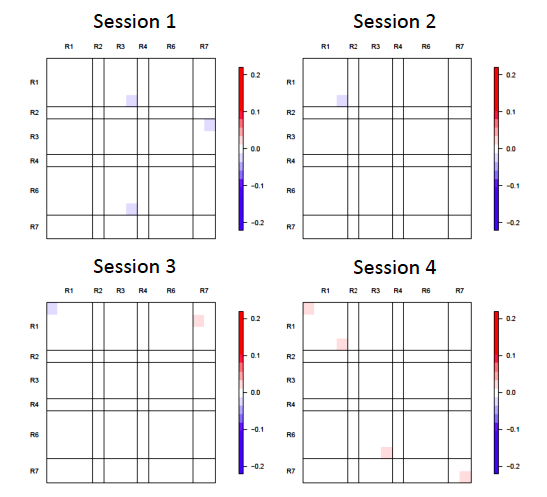
\includegraphics[width=5in]{session.png}
				\label{session}
			\end{figure} 
			\clearpage}
		
		\afterpage{
			\begin{figure}[h]
				\caption{Posterior modes of subject-level effects for 15 ROI's across 7 brain networks for the first 4 subjects in the dataset}
				\centering
				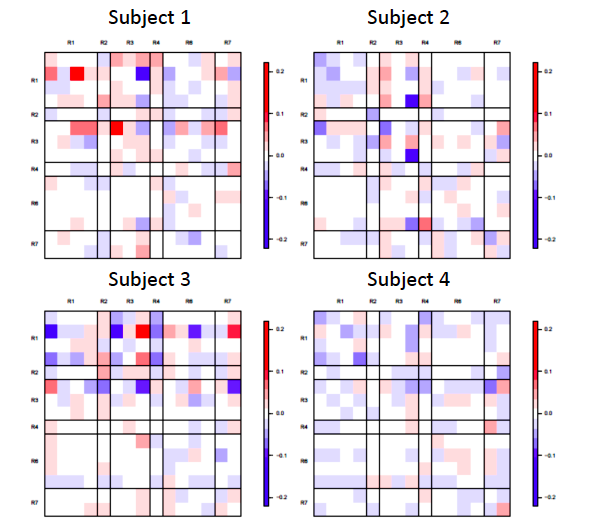
\includegraphics[width=5in]{subject.png}
				\label{subject}
			\end{figure} 
			\clearpage}
		
		\afterpage{
			\begin{figure}[h]
				\caption{Posterior modes of session-level standard deviation, subject-level standard deviation and the ratio of session-level variance over the sum of session- and subject-level variances}
				\centering
				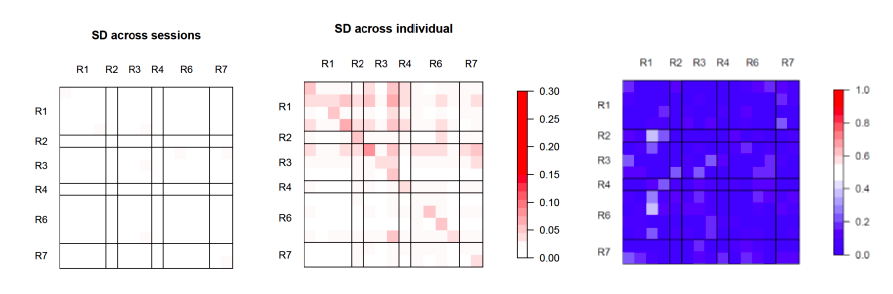
\includegraphics[width=6in]{variability.png}
				\label{variability}
			\end{figure} 
			\clearpage}
		
		
		
		
		\section{References}
		
		\begin{thebibliography}{9}
			
			\bibitem{Gefang} 
			Gefang D.
			\textit{Bayesian doubly adaptive elastic-net LASSO for VAR shrinkage}. 
			International Journal of Forecasting 30 1-11 (2014).
			
			
			\bibitem{Gorrostieta} 
			Gorrostieta G, Fiecas M, Ombao H, Burke E, Cramer S.
			\textit{Hierarchical vector auto-regressive models and their applications to multi-subject effective connectivity}. 
			Frontiers in Computational Neuroscience 7 (2013).
			
			
			\bibitem{Harrison} 
			Harrison L, Penny WD, Friston K.
			\textit{Multivariate autoregressive modeling of fMRI time series}. 
			NeuroImage (2003).
			
			
			
			\bibitem{Lin} 
			Li Q, Lin N.
			\textit{New introduction to multiple time series analysis}. 
			Berlin; Heidelberg; New York, NY: Springer-Verlag (2005).
			
			
			\bibitem{Park} 
			Park T, Casella G.
			\textit{The Bayesian Lasso}. 
			JASA Vol.103, No.482 (2008).
			
			
			
			\bibitem{Scott} 
			Scoot SL, Blocker AW, Bonassi FV.
			\textit{Bayes and big data: The consensus Monte Carlo algorithm}. 
			Bayes (2013).
			
			
		\end{thebibliography}
		
		
		
	\end{document}